% !TEX root = ../main.tex
\begin{table}[t]
    \centering
    \resizebox{\textwidth}{!}{
    \begin{tabular}{l|c|c|c|c}
    Models                    & 1-shot Acc.         & 5-shot Acc.         & 1-shot Acc. w/ D    & 5-shot Acc. w/ D     \\
    \hline\hline
    Supervised                & 46.52 $\pm$ 0.52    & 66.15 $\pm$ 0.22    & 46.52 $\pm$ 0.52    & 66.15 $\pm$ 0.22     \\
    \hline
    Semi-Supervised Inference & 50.74 $\pm$ 0.75    & 69.37 $\pm$ 0.26    & 48.67 $\pm$ 0.60    & 67.46 $\pm$ 0.24      \\
    \hline\hline
    Soft $k$-Means            & 51.52 $\pm$ 0.36    &\tb{70.25 $\pm$ 0.31}& 49.88 $\pm$ 0.52    & 68.32 $\pm$ 0.22     \\
    \hline
    Soft $k$-Means+Cluster    &\tb{51.85 $\pm$ 0.25}& 69.42 $\pm$ 0.17    &\tb{51.36 $\pm$ 0.31}& 67.56 $\pm$ 0.10     \\
    \hline
    Masked Soft $k$-Means     &\tb{52.39 $\pm$ 0.44}&\tb{69.88 $\pm$ 0.20}&\tb{51.38 $\pm$ 0.38}&\tb{69.08 $\pm$ 0.25} \\
    \end{tabular}
    }
    \caption{\textit{tiered}ImageNet 1/5-shot classification results. ``w/ D'' denotes ``with
    distractors'' where the unlabeled images contain irrelevant classes.}
    \label{tab:tieredImageNet}
\end{table}
\begin{figure}
    \centering
    \iflatexml
    \includegraphics[width=\textwidth]{figures/tnet_num_unlabel.png}
    \else
    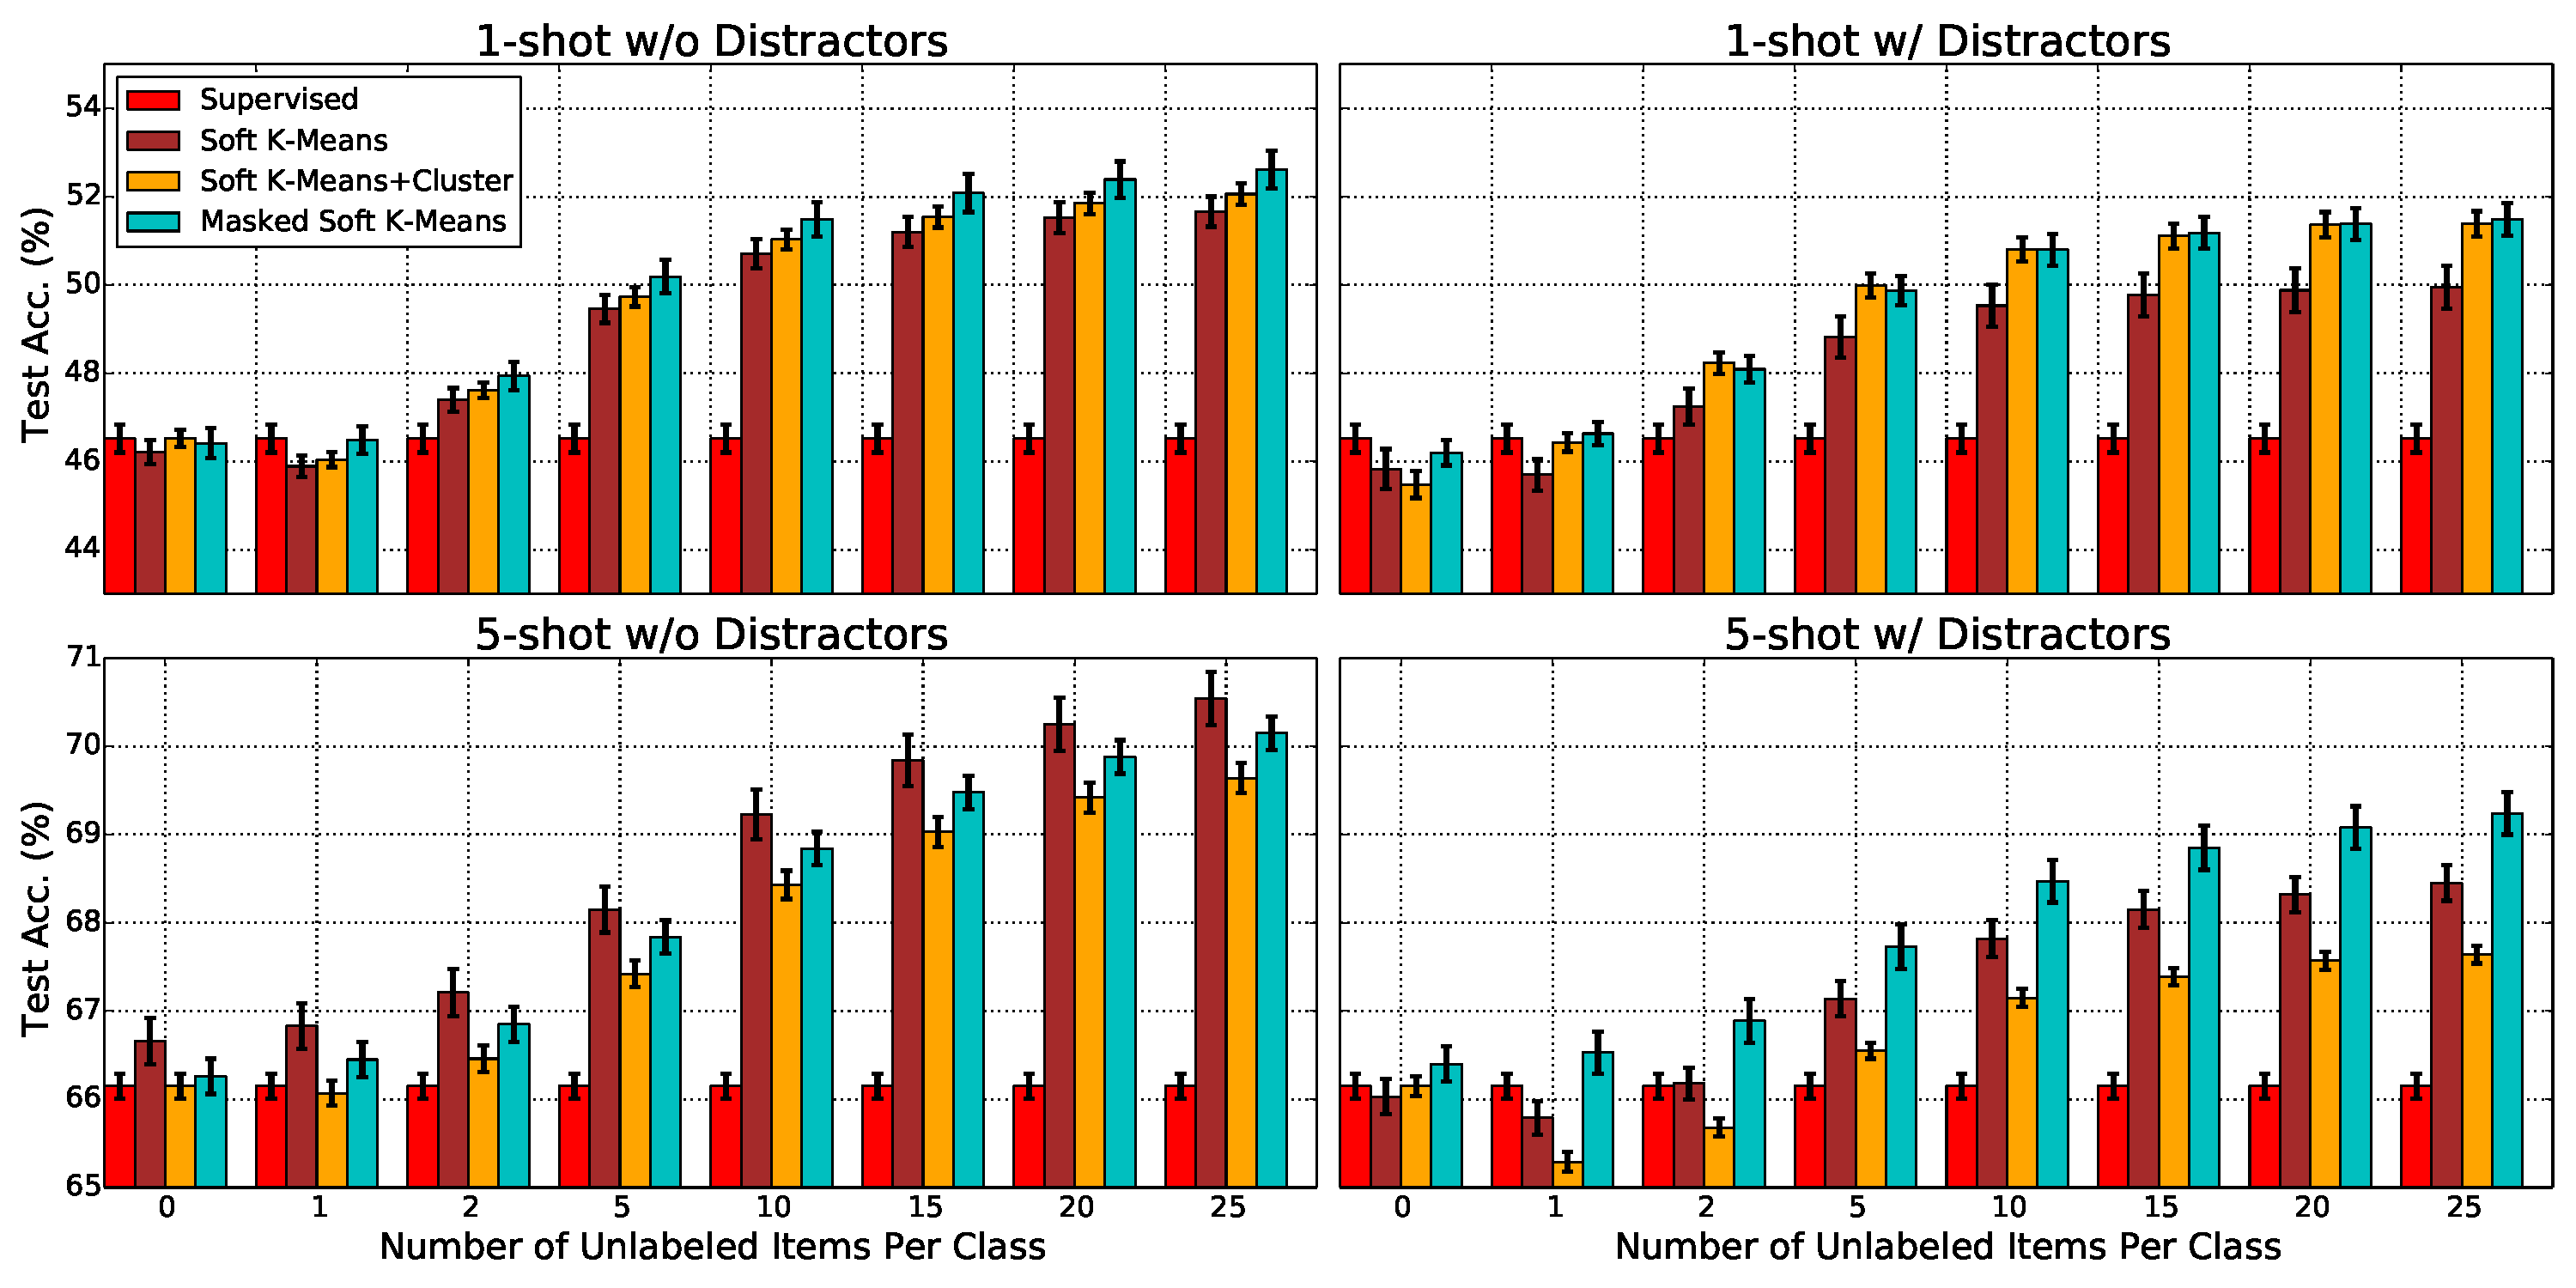
\includegraphics[width=\textwidth]{figures/tnet_num_unlabel.pdf}
    \fi
    \caption{Model Performance on {\it tiered}ImageNet with different number of unlabeled items during test time.}
    \label{fig:tnet_num_unlabel}
\end{figure}